%\VignetteIndexEntry{Introduction to the dataRetrieval package}
%\VignetteEngine{knitr::knitr}
%\VignetteDepends{}
%\VignetteSuggests{xtable}
%\VignetteImports{XML, RCurl, reshape2,lubridate,httr,plyr}
%\VignettePackage{dataRetrieval}

\documentclass[a4paper,11pt]{article}\usepackage[]{graphicx}\usepackage[]{color}
%% maxwidth is the original width if it is less than linewidth
%% otherwise use linewidth (to make sure the graphics do not exceed the margin)
\makeatletter
\def\maxwidth{ %
  \ifdim\Gin@nat@width>\linewidth
    \linewidth
  \else
    \Gin@nat@width
  \fi
}
\makeatother

\definecolor{fgcolor}{rgb}{0.345, 0.345, 0.345}
\newcommand{\hlnum}[1]{\textcolor[rgb]{0.686,0.059,0.569}{#1}}%
\newcommand{\hlstr}[1]{\textcolor[rgb]{0.192,0.494,0.8}{#1}}%
\newcommand{\hlcom}[1]{\textcolor[rgb]{0.678,0.584,0.686}{\textit{#1}}}%
\newcommand{\hlopt}[1]{\textcolor[rgb]{0,0,0}{#1}}%
\newcommand{\hlstd}[1]{\textcolor[rgb]{0.345,0.345,0.345}{#1}}%
\newcommand{\hlkwa}[1]{\textcolor[rgb]{0.161,0.373,0.58}{\textbf{#1}}}%
\newcommand{\hlkwb}[1]{\textcolor[rgb]{0.69,0.353,0.396}{#1}}%
\newcommand{\hlkwc}[1]{\textcolor[rgb]{0.333,0.667,0.333}{#1}}%
\newcommand{\hlkwd}[1]{\textcolor[rgb]{0.737,0.353,0.396}{\textbf{#1}}}%

\usepackage{framed}
\makeatletter
\newenvironment{kframe}{%
 \def\at@end@of@kframe{}%
 \ifinner\ifhmode%
  \def\at@end@of@kframe{\end{minipage}}%
  \begin{minipage}{\columnwidth}%
 \fi\fi%
 \def\FrameCommand##1{\hskip\@totalleftmargin \hskip-\fboxsep
 \colorbox{shadecolor}{##1}\hskip-\fboxsep
     % There is no \\@totalrightmargin, so:
     \hskip-\linewidth \hskip-\@totalleftmargin \hskip\columnwidth}%
 \MakeFramed {\advance\hsize-\width
   \@totalleftmargin\z@ \linewidth\hsize
   \@setminipage}}%
 {\par\unskip\endMakeFramed%
 \at@end@of@kframe}
\makeatother

\definecolor{shadecolor}{rgb}{.97, .97, .97}
\definecolor{messagecolor}{rgb}{0, 0, 0}
\definecolor{warningcolor}{rgb}{1, 0, 1}
\definecolor{errorcolor}{rgb}{1, 0, 0}
\newenvironment{knitrout}{}{} % an empty environment to be redefined in TeX

\usepackage{alltt}

\usepackage{amsmath}
\usepackage{times}
\usepackage{hyperref}
\usepackage[numbers, round]{natbib}
\usepackage[american]{babel}
\usepackage{authblk}
\usepackage{subfig}
\usepackage{placeins}
\usepackage{footnote}
\usepackage{tabularx}
\usepackage{threeparttable}
\usepackage{parskip}

\usepackage{csquotes}
\usepackage{setspace}

% \doublespacing

\renewcommand{\topfraction}{0.85}
\renewcommand{\textfraction}{0.1}
\usepackage{graphicx}


\usepackage{mathptmx}% Times Roman font
\usepackage[scaled=.90]{helvet}% Helvetica, served as a model for arial

% \usepackage{indentfirst}
% \setlength\parindent{20pt}
\setlength{\parskip}{0pt}

\usepackage{courier}

\usepackage{titlesec}
\usepackage{titletoc}

\titleformat{\section}
  {\normalfont\sffamily\bfseries\LARGE}
  {\thesection}{0.5em}{}
\titleformat{\subsection}
  {\normalfont\sffamily\bfseries\Large}
  {\thesubsection}{0.5em}{}
\titleformat{\subsubsection}
  {\normalfont\sffamily\large}
  {\thesubsubsection}{0.5em}{}
  
\titlecontents{section}
[2em]                 % adjust left margin
{\sffamily}             % font formatting
{\contentslabel{2.3em}} % section label and offset
{\hspace*{-2.3em}}
{\titlerule*[0.25pc]{.}\contentspage}
  
\titlecontents{subsection}
[4.6em]                 % adjust left margin
{\sffamily}             % font formatting
{\contentslabel{2.3em}} % section label and offset
{\hspace*{-2.3em}}
{\titlerule*[0.25pc]{.}\contentspage}
  
\titlecontents{subsubsection}
[6.9em]                 % adjust left margin
{\sffamily}             % font formatting
{\contentslabel{2.3em}} % section label and offset
{\hspace*{-2.3em}}
{\titlerule*[0.25pc]{.}\contentspage}

\titlecontents{table}
[0em]                 % adjust left margin
{\sffamily}             % font formatting
{Table\hspace*{2em} \contentslabel {2em}} % section label and offset
{\hspace*{4em}}
{\titlerule*[0.25pc]{.}\contentspage}

\titlecontents{figure}
[0em]                 % adjust left margin
{\sffamily}             % font formatting
{Figure\hspace*{2em} \contentslabel {2em}} % section label and offset
{\hspace*{4em}}
{\titlerule*[0.25pc]{.}\contentspage}

%Italisize and change font of urls:
\urlstyle{sf}
\renewcommand\UrlFont\itshape

\usepackage{caption}
\captionsetup{
  font={sf},
  labelfont={bf,sf},
  labelsep=period,
  justification=justified,
  singlelinecheck=false
}



\textwidth=6.2in
\textheight=8.5in
\parskip=.3cm
\oddsidemargin=.1in
\evensidemargin=.1in
\headheight=-.3in


%------------------------------------------------------------
% newcommand
%------------------------------------------------------------
\newcommand{\scscst}{\scriptscriptstyle}
\newcommand{\scst}{\scriptstyle}
\newcommand{\Robject}[1]{{\texttt{#1}}}
\newcommand{\Rfunction}[1]{{\texttt{#1}}}
\newcommand{\Rclass}[1]{\textit{#1}}
\newcommand{\Rpackage}[1]{\textit{#1}}
\newcommand{\Rexpression}[1]{\texttt{#1}}
\newcommand{\Rmethod}[1]{{\texttt{#1}}}
\newcommand{\Rfunarg}[1]{{\texttt{#1}}}
\IfFileExists{upquote.sty}{\usepackage{upquote}}{}
\begin{document}



\renewenvironment{knitrout}{\begin{singlespace}}{\end{singlespace}}
\renewcommand*\listfigurename{Figures}

\renewcommand*\listtablename{Tables}


%------------------------------------------------------------
\title{The dataRetrieval R package}
%------------------------------------------------------------
\author[1]{Laura A. De Cicco}
\author[1]{Robert M. Hirsch}
\affil[1]{United States Geological Survey}




\noindent{\huge\textsf{\textbf{The dataRetrieval R package}}}

\noindent\textsf{By Laura A. De Cicco and Robert M. Hirsch}

\noindent\textsf{\today}

\begin{center}
U.S. DEPARTMENT OF THE INTERIOR - U.S. GEOLOGICAL SURVEY - WATER RESOURCES\\
 STATION:06934500 Missouri River at Hermann, MO TYPE:STREAM AGENCY:USGS STATE:29 COUNTY:139
 LATITUDE: 384235.3 LONGITUDE: 0912618.6 NAD83 DRAINAGE AREA:522500 CONTRIBUTING DRAINAGE AREA: DATUM:481.50 NAVD88
 Date Processed:  By swreview
 INPUT DD: Gage height FROM THE DCP (ft)
 PROVISIONAL DATA FOR PERIOD 10/01/2012 to 09/30/2013
 MAXIMUM FOR PERIOD, BASED ON 365 EQUIVALENT DAYS OF RECORD.
 TIME DISCHARGE Gage height
 DATE HH MM SS (CFS) (CMS) (FT) (M)
---------- -------- ----- ----- ----- -----
 *** NO VALID BASE DISCHARGE AVAILABLE ***
MAXIMUM INSTANTANEOUS DISCHARGE AND CORRESPONDING Gage height
06/01/2013 21:30:00 457000 13000 33.14 10.10
MINIMUM INSTANTANEOUS DISCHARGE AND CORRESPONDING Gage height
01/29/2013 13:15:00 26600 753 0.93 0.28
MAXIMUM INSTANTANEOUS Gage height AND CORRESPONDING DISCHARGE
06/01/2013 21:30:00 457000 13000 33.14 10.10
MINIMUM INSTANTANEOUS Gage height AND CORRESPONDING DISCHARGE
01/29/2013 13:15:00 26600 753 0.93 0.28
MAXIMUM DAILY DISCHARGE
06/02/2013 435000 12300
MINIMUM DAILY DISCHARGE
01/29/2013 26900 762
\end{center}
Example text outside R code here; we know the value of pi is 3.142.

\begin{knitrout}
\definecolor{shadecolor}{rgb}{0.969, 0.969, 0.969}\color{fgcolor}\begin{kframe}
\begin{alltt}
\hlkwd{set.seed}\hlstd{(}\hlnum{1213}\hlstd{)}  \hlcom{# for reproducibility}
\hlstd{x} \hlkwb{=} \hlkwd{cumsum}\hlstd{(}\hlkwd{rnorm}\hlstd{(}\hlnum{100}\hlstd{))}
\hlkwd{mean}\hlstd{(x)}  \hlcom{# mean of x}
\end{alltt}
\begin{verbatim}
[1] -1.939758
\end{verbatim}
\begin{alltt}
\hlkwd{plot}\hlstd{(x,} \hlkwc{type} \hlstd{=} \hlstr{'l'}\hlstd{)}  \hlcom{# Brownian motion}
\end{alltt}
\end{kframe}
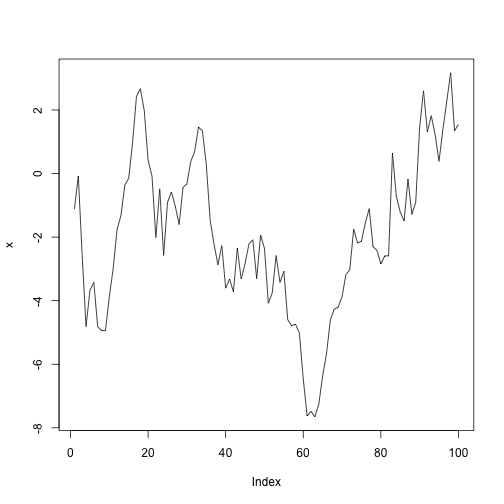
\includegraphics[width=\maxwidth]{figure/my-label-1} 

\end{knitrout}


\end{document}
